\begin{frame}{Juste des suppositions}
  Devinons le genre de chaque mot ci-dessous en donnant le bon article (\lexi{le} ou \lexi{la}).
  Il est peu probable que vous savez ces mots, alors il faut deviner selon les terminaisons.
  \begin{columns}[b]
    \column{0.3\textwidth}
      \begin{center}
        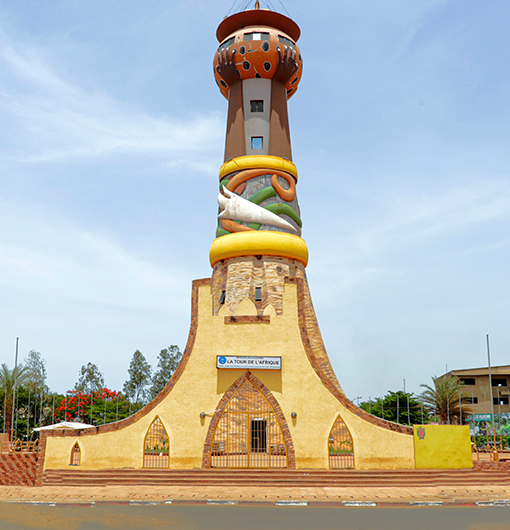
\includegraphics[scale=0.18]{bamako.jpg} \\
        \underline{\uncover<2->{La}} \alert{tour} de l'Afrique à Bamako au Mali
      \end{center}
    \column{0.3\textwidth}
      \begin{center}
        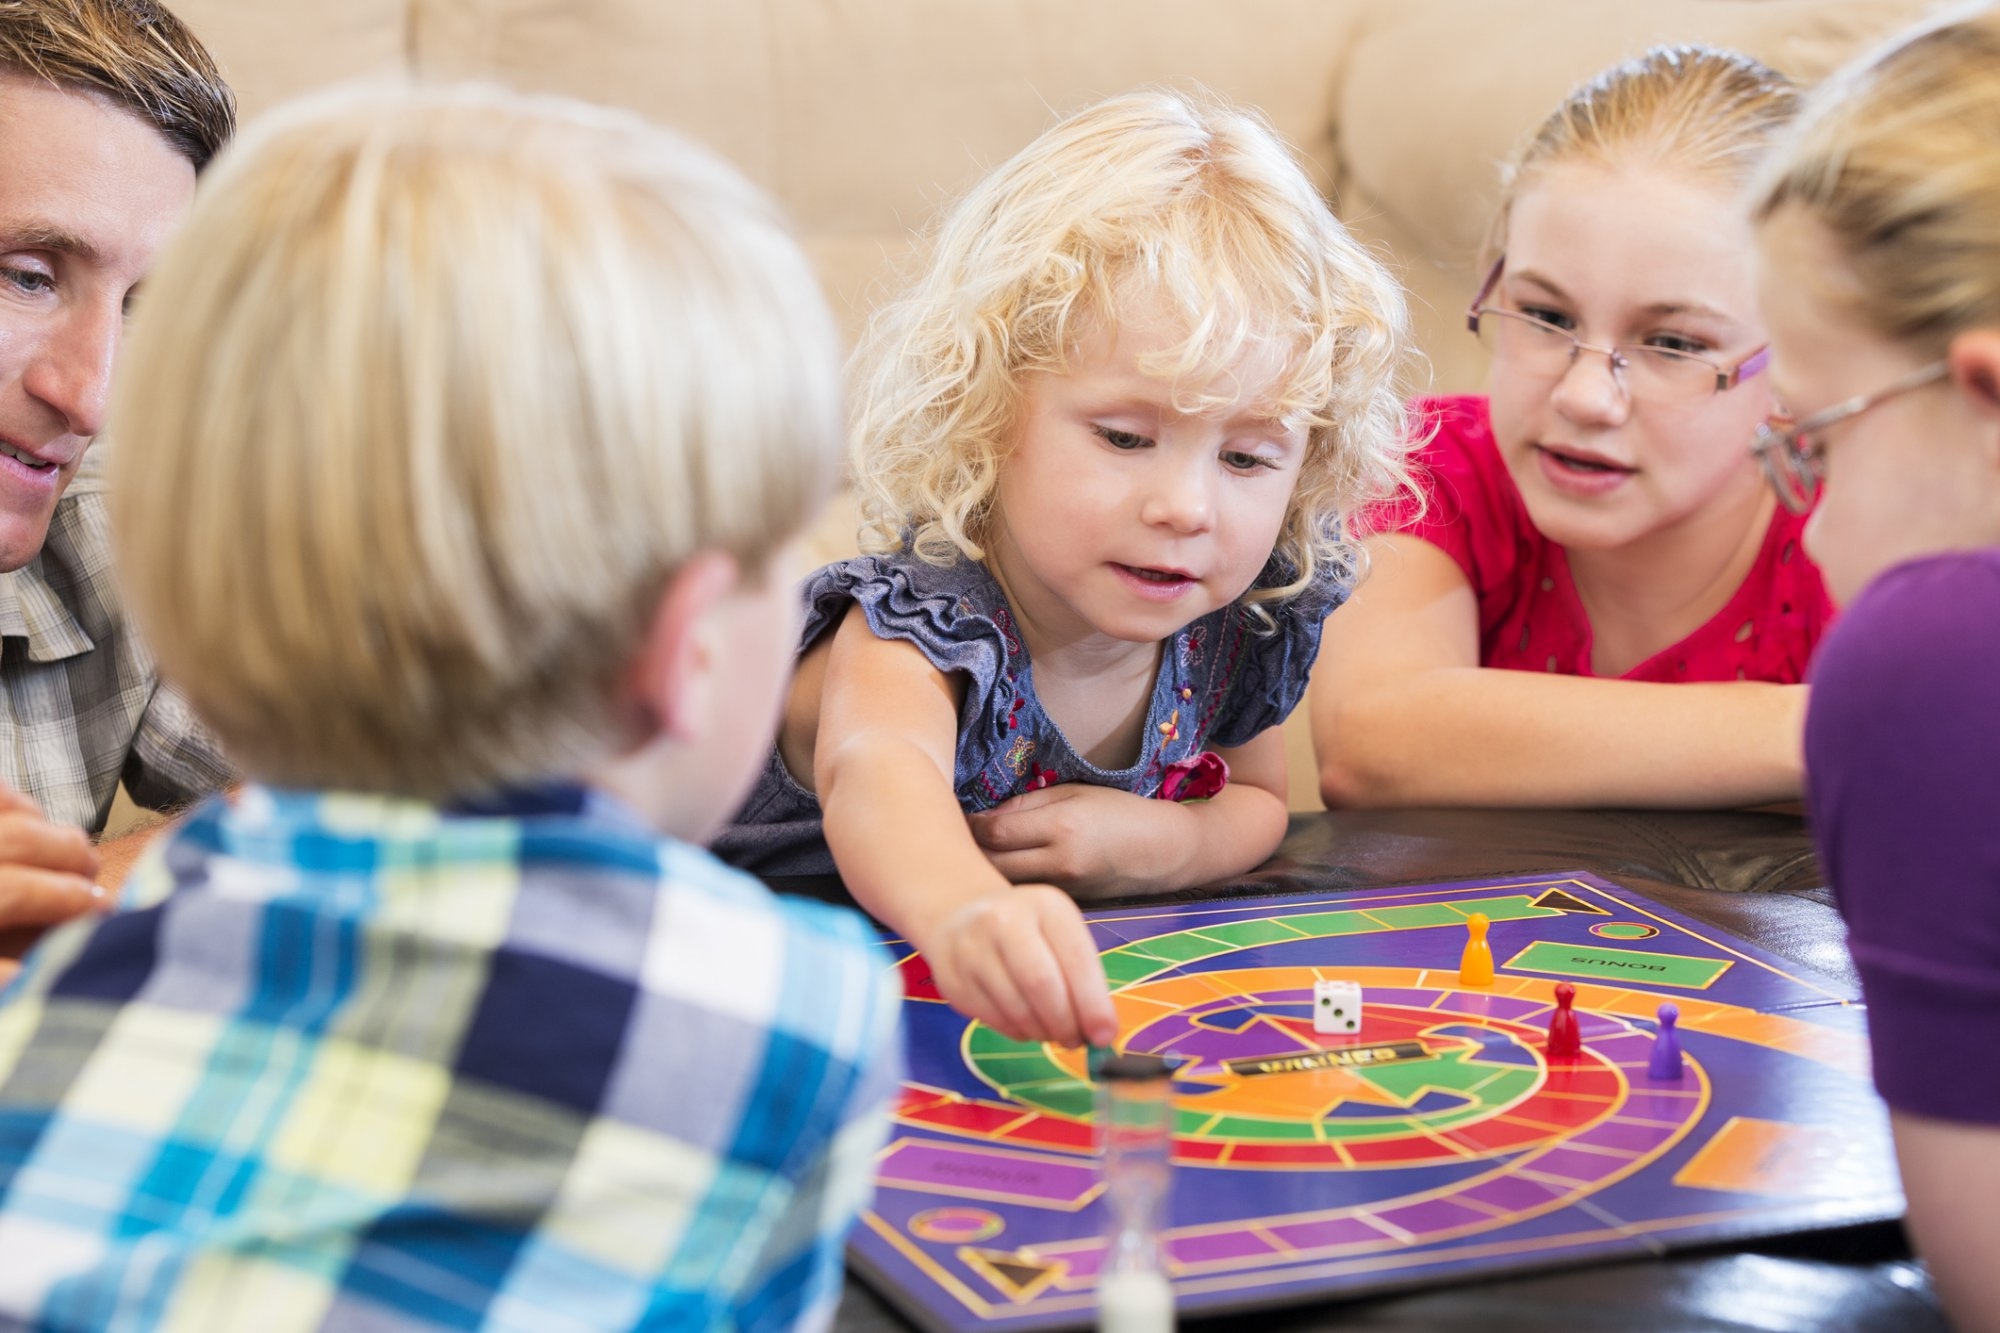
\includegraphics[scale=0.07]{jeudesociete.jpg} \\
        \underline{\uncover<2->{Un}} \alert{tour} dans un jeu de société
      \end{center}
    \column{0.4\textwidth}
      \begin{enumerate}
        \item \underline{\uncover<3->{la}} galaxie
        \item \underline{\uncover<4->{la}} suppression
        \item \underline{\uncover<5->{le}} dossier
        \item \underline{\uncover<6->{le}} sceau
        \item \underline{\uncover<7->{l'}} échappement \uncover<8->{(m.)}
        \item \underline{\uncover<9->{le}} prisme
        \item \underline{\uncover<10->{la}} brochure
        \item \underline{\uncover<11->{le}} repassage
        \item \underline{\uncover<12->{la}} réalité
      \end{enumerate}
  \end{columns}
\end{frame}